Conforme identificado na elicitação de requisitos, uma das funcionalidades requeridas para a plataforma é a geração de boletins meteorológicos diários, detalhados anteriormente na Seção \ref{sec:boletim}.

Embora esta funcionalidade deva ser implementada em uma etapa posterior, conforme exposto na Seção \ref{sec:agenda}, foi identificada a necessidade de realizar uma especificação do mesmo junto ao cliente, elaborando uma visualização e estabelecendo os elementos que o mesmo deveria apresentar. Como resultado, tem-se o modelo apresentado na Figura \ref{fig:modeloBoletim}, que contempla a data, precipitação, temperaturas máxima e mínima, índice de calor, rajada e sua classificação na Escala de Beaufort, e ainda a logomarca do LabInstru e da Universidade do Estado do Amazonas.

\newpage

\begin{figure}[h!]
	\centering
	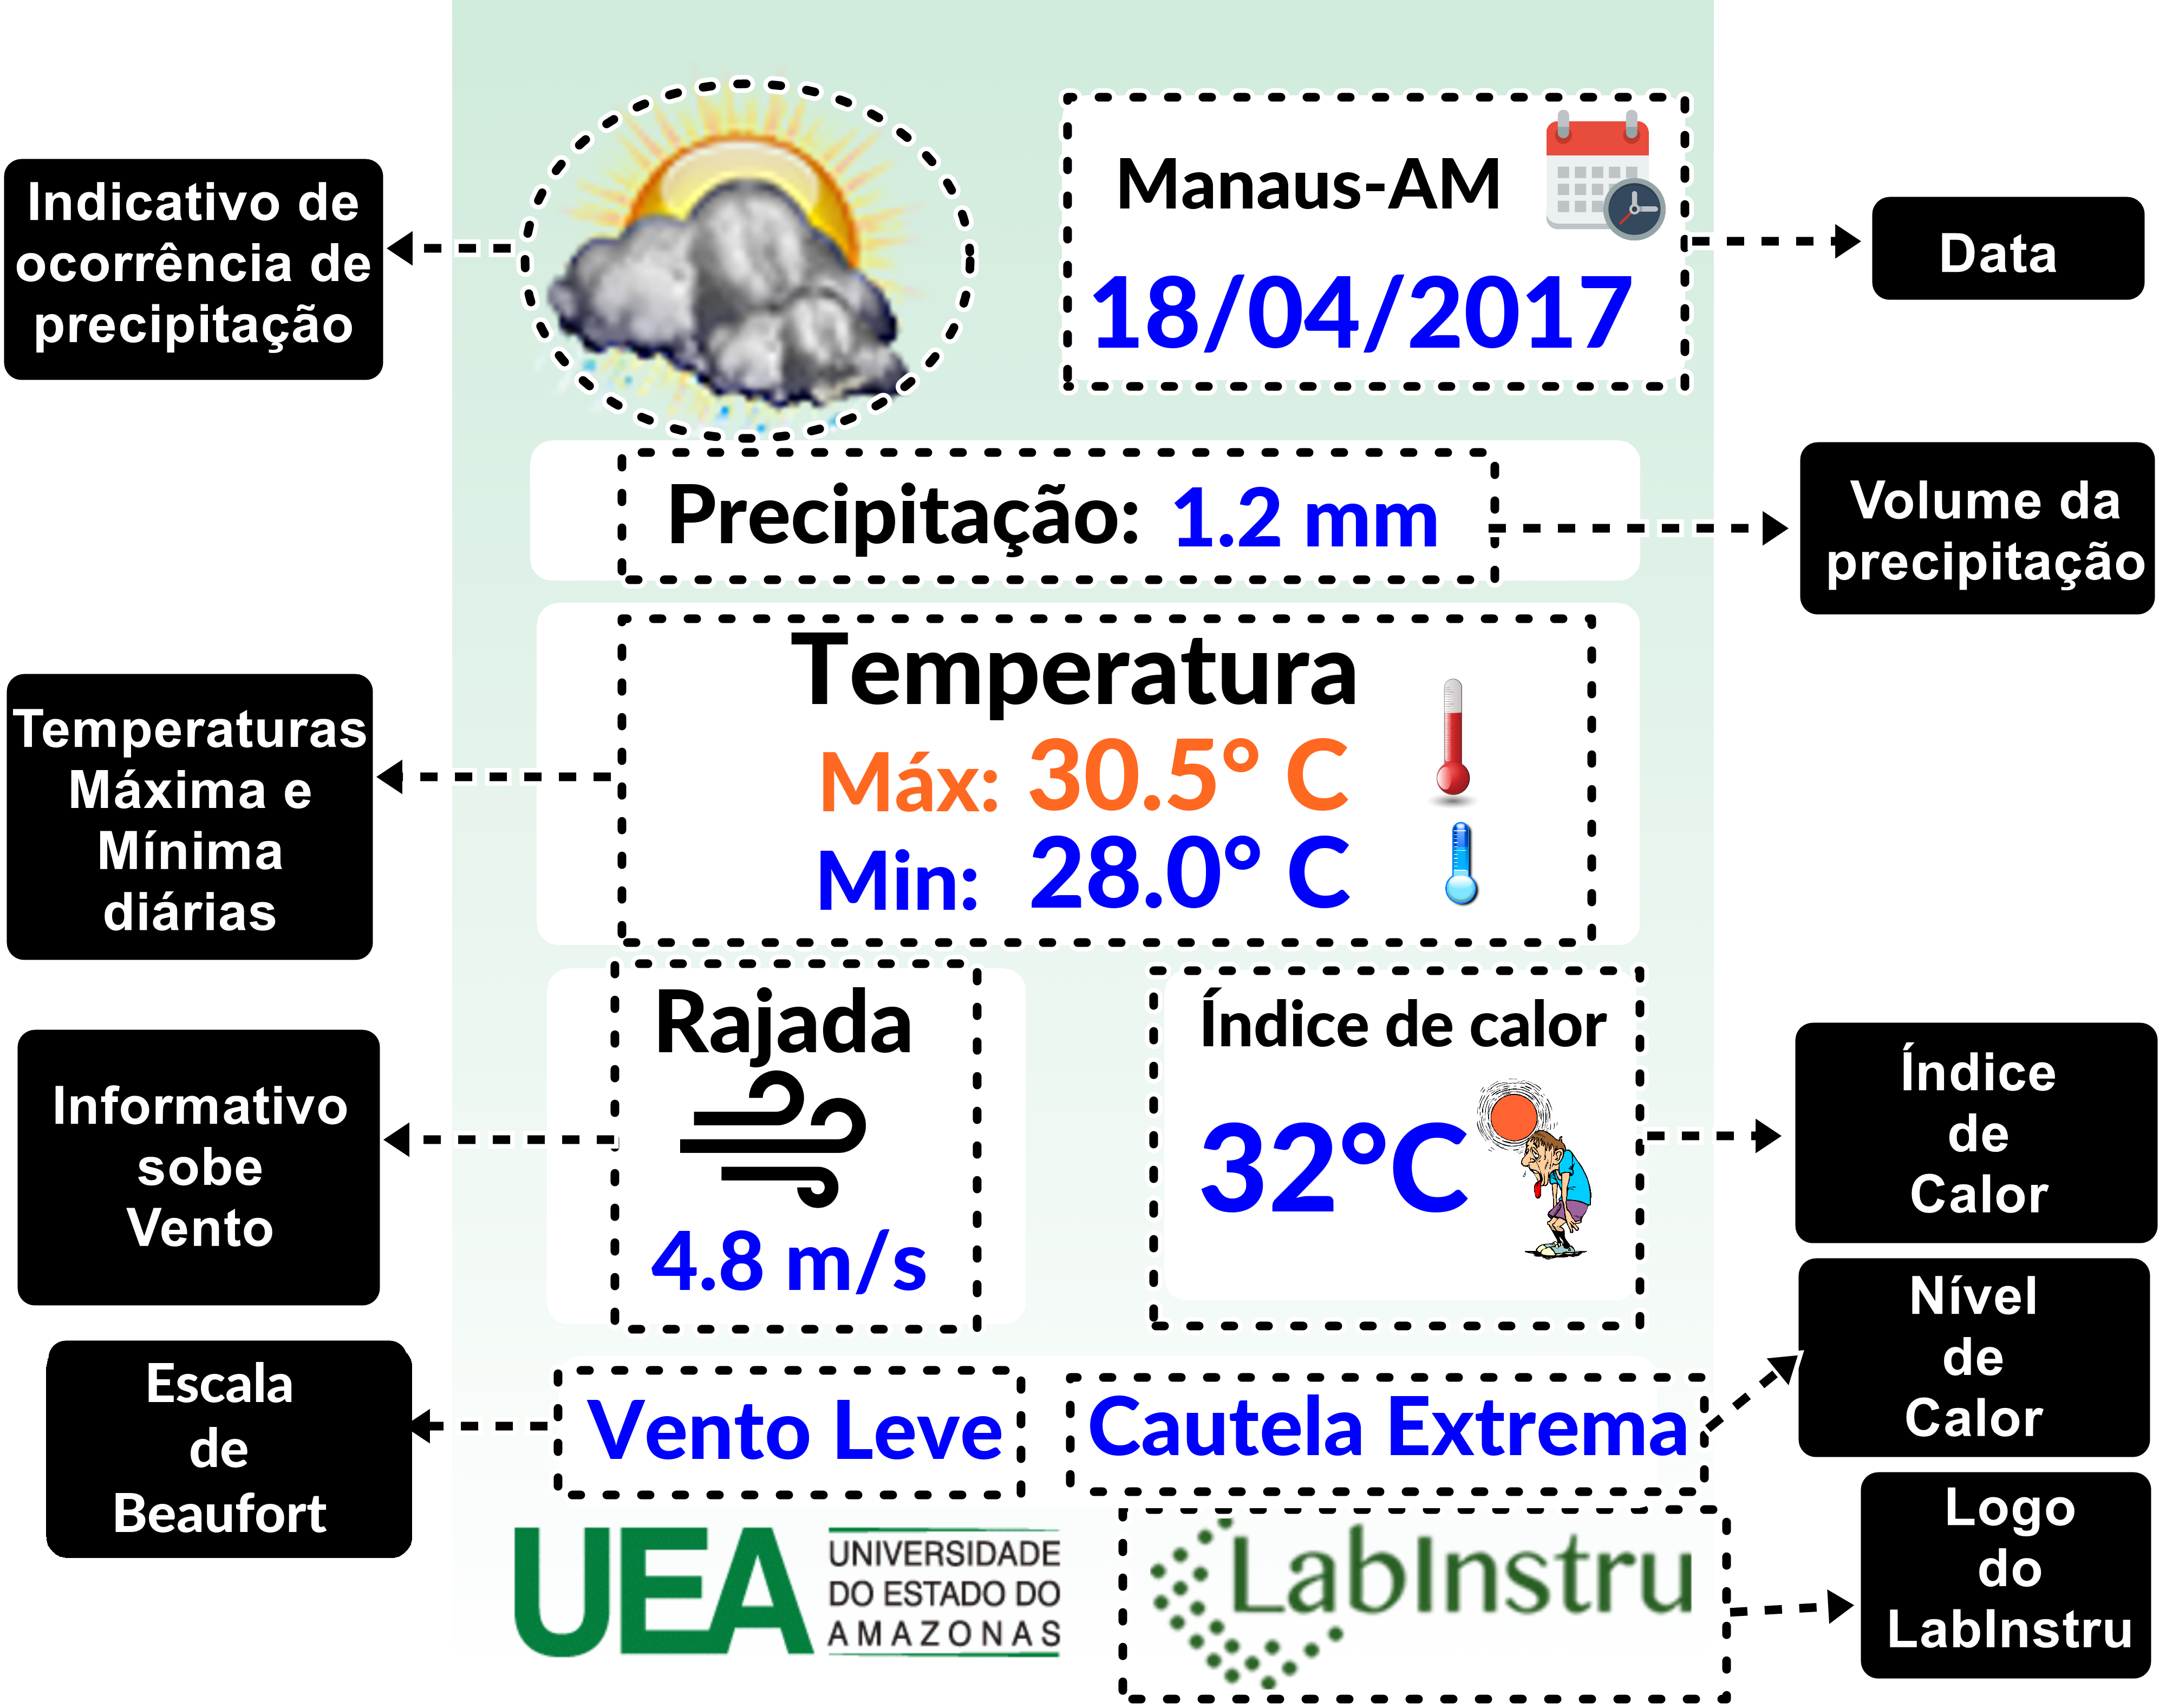
\includegraphics[width=0.9\textwidth]{./img/esbocoBoletim.png}
	\caption{Modelo referente ao boletim meteorológico gerado pelo LabInstru Web. Fonte: Próprio autor.} \label{fig:modeloBoletim}
\end{figure}

Produzir este modelo automaticamente a partir dos dados contidos na aplicação será uma das etapas posteriores deste trabalho.
